\documentclass[conference]{IEEEtran}
\IEEEoverridecommandlockouts

\usepackage{cite}
\usepackage{amsmath,amssymb,amsfonts}
\usepackage{graphicx}
\usepackage{textcomp}
\usepackage{xcolor}
\usepackage{booktabs}
\usepackage{multirow}
\usepackage{enumitem}
\usepackage{url}
\usepackage{float}
\usepackage{stfloats}
\usepackage[hidelinks]{hyperref}

\begin{document}

\title{Finding a Hamiltonian Latent Space for Gravitational Wave Representation}

\author{\IEEEauthorblockN{Aleksandr Beliaev}
\IEEEauthorblockA{\textit{University of Toronto} \\
Toronto, Canada \\
aleksandr.beliaev@mail.utoronto.ca}
}

\maketitle

\section{Introduction}

This paper introduces empirical study of gravitational wave representation via physics-informed deep learning and a novel methodoligical variance-based approach. We model binary black hole (BBH) inspirals as an energy dissapative Hamiltonian system during the pre-merger regime. We train 3 Hamiltonian-regularized convolutional auto-encoders (CAE), a variational Hamiltonian auto-encoder (VH-AE), a Hamiltonian auto-encoder (H-AE), and a Port-Hamiltonian auto-encoder (PHAE), as well as a parameter-matched CAE on synthetic BBH inspiral waveforms. 
We demonstrate that a physically motivated representation improves out-of-distribution generalization, parameter estimation, and yields a more structured latent space. The variational loss demonstrates that these improvements can be achivied with nearly the same training cost as the CAE. 
% ===========================================================================
\section{Introduction}
The motivation behind this project is to apply a physics-informed loss function to gravitational-wave modeling and test whether it improves generalization to out-of-distribution signals. Binary black hole (BBH) inspirals radiate gravitational waves whose orbital dynamics can be modelled as an energy-conservative system during the pre-merger regime, making them a natural testbed for Hamiltonian inductive biases. I train a Hamiltonian-regularized convolutional autoencoder (H-AE) on synthetic BBH inspiral waveforms and evaluate it against an architecturally identical convolutional autoencoder (CAE) baseline along three axes:
\begin{itemize}
\item reconstruction and generalization to a held-out high-mass BBH regime;
\item emergence of Hamiltonian structure in the learned latent space.
\item effect of the relative weight of the physics loss function on the above.
\end{itemize}

% ===========================================================================

\section{Full Hamiltonian Derivation}

We approximate two Binary Black Holes (BBH) as two masses rotating around a centre of mass kept in place by angular momentum. This reduces the problem to a fictious particle with a relative separation:

\begin{equation}
\mu = \frac{m_1 m_2}{m_1 + m_2}, \qquad M = m_1 + m_2
\end{equation}
For this system, $H$ is a known function over all of phase space

\begin{equation}
\H = \frac{\|P\|^2}{2 \mu} - \frac{G \mu M}{\|q\|}
\end{equation}

where a contour defines an energy level. 

\section{Physics and Machine Learning Background}

Gravitational waves were originally predicted by Einstein's general theory of relativity all the way back in 1916, yet were only measured for the first time in 2015 by the NSF LIGO observatory \cite{LIGOLabGW}. The Laser Interferometer Gravitational-Wave Observatory (LIGO) is the primary gravitational wave observatory. The only kind of waves detected by LIGO have been Compact Binary Inspiral Gravitational Waves caused by either 2 neutron stars, 2 black holes, or a black hole and a neutron star orbiting each other until they collide\cite{LIGOLabSources}. As the objects start orbiting each other, they emit gravitational waves, losing energy, coming closer together, rotating quicker and quicker, releasing gravitational waves. 

\begin{equation}
\frac{dH}{dt} =
\frac{\partial H}{\partial q}\dot{q}
+ \frac{\partial H}{\partial p}\dot{p}
= 0.
\end{equation}

Machine learning approaches have become the industry standard in gravitational wave detection, with end-to-end low latency pipeline operational in production settings \cite{Marx2024}\cite{Benoit2025}. These approaches were developed on the initial demonstration of deep convolutional learning at matching status quo method's sensitivity \cite{George2018}. Gravitational waves have also been shown to form a signal manifold on a low-dimensional space\cite{Magee2024}. This suggests that a compact latent representation is not only possible but is also physically informed. Additionally, Hamiltonian Neural Networks learn a scalar energy function whose symplectic gradient matches observed dynamics\cite{Greydanus2019}. Hamiltonian Generative Networks extend this approach to high-dimensional observations by learning the Hamiltonian in latent space inferred by an encoder\cite{Toth2020}. \\

To my knowledge, these two threads have not been combined. It remains an open question whether the inspiral stage of a BBH admits a useful Hamiltonian representation in the latent space of an encoder. This project is a direct empirical test of this hypothesis.

% ===========================================================================
\section{Data Generation and Processing}
As stated in the introduction, both the input and target for the HAE and CAE are the clean waveform signal of a BBH merger.
\begin{figure}[h]
    \centering
    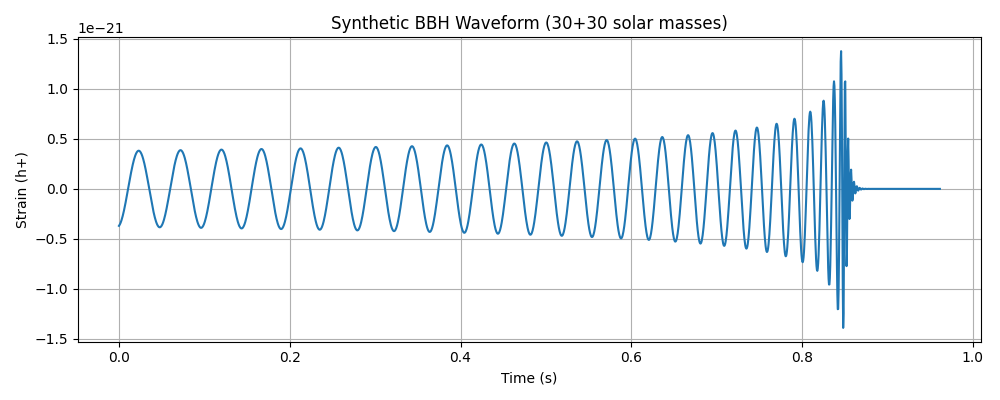
\includegraphics[width=\linewidth]{figures/BBHchirp.png}
    \caption{Synthetically generated classical chirp of a binary black hole in-spiral and merger. Increasing frequency and amplitude increase up-to the peak at merger and then settle rapidly. Both black holes have the mass of 30 suns.}
    \label{fig:whitened_injection}
\end{figure}

The data generation and processing pipeline.
\begin{itemize}
\item Synthetic BBH injections of masses between 20 and 80 $M \odot$ are generated with PyCBC and stored in a HDF5 file using the ggwd pipeline\cite{Gebhard2019}. Synthetic signal for each sample contains the H1 waveform, H1 whitened strain, and wave parameters (mass1, mass2, spins, SNR, location).

\item The signal is cropped to the inspiral regime. Out of 8 seconds of generated signal at 2048 Hz, a 1792-sample (\~0.87(s)) window is taken 256 samples (\~0.125(s)) before the merger.
\item Each cropped waveform is normalized, yielding $O(1)$ amplitudes across the dataset.
\end{itemize}
The data is split up such that the model never sees heavy BBH waveforms during training. An RNG seed controls the train/validation partition and shuffle was set to false to make reported metrics deterministic.
\begin{itemize}
\item Training (1073 samples) and validation sets are assigned all BBH signals with both component masses $\le 60 M \odot$.
\item Validation (189 samples) is a random 15\% holdout of the training range.
\item Testing set (79 samples) is comprised of both masses $\geq 70 M \odot$.
\end{itemize}

% ===========================================================================
\section{Architecture}
A key motivation in the design of the architecture was controlled comparison. The project was focused on the effect of the Hamiltonian loss function, so the encoder architecture (outside of the latent dimensionality) was fixed.
\begin{figure}[t]
    \centering
    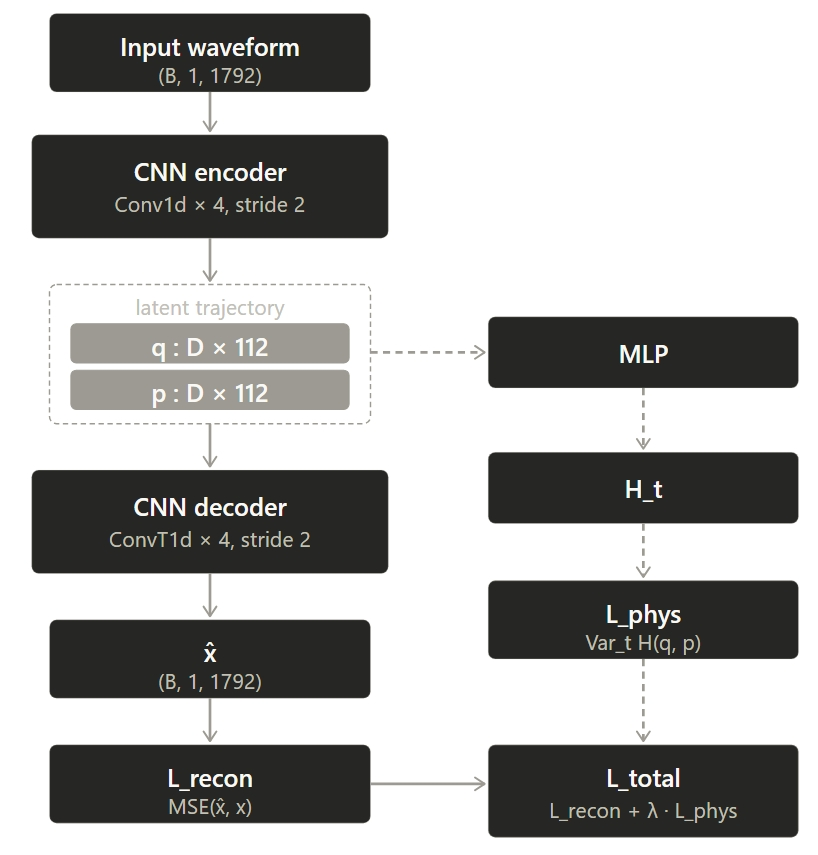
\includegraphics[width=\linewidth]{figures/Architecture_SVG.png}
    \caption{Architecture diagram for the HAE. The CAE is exactly alike just without the Hamiltonian MLP and Loss.}
    \label{fig:architecture}
\end{figure}

\subsection{Encoder, Latent Space, and Decoder}

Four strided Conv1d blocks (kernel 5, stride 2, GroupNorm) with channels 1, 16, 32, 64, 128 are followed with a 1 by 1 projection into $2 \times latent\_dim$ channels. The temporal dimension halves every block from 1792 to 112.

The $2 \times latent\_dim$ channels are split along the channel axis into $q$ and $p$, canonical position and momentum. There are 112 $q$ and $p$ vectors in the latent dimension representing 112 latent timesteps.

Decoder mirrors the encoder. a 1 by 1 projection back to 128 channels, followed by three ConvTranspose1d blocks and a final transpose-conv to recover (B, 1, 1792). The output padding set to 1 guarantees exact 2 times up scaling.

The CAE reconstruction MSE loss is given by
\begin{equation}
\mathcal{L}_{\text{recon}} \;=\; \frac{1}{B \cdot T_x} \sum_{b=1}^{B} \sum_{t=1}^{T_x} \bigl( \hat{x}_{b,t} - x_{b,t} \bigr)^{2}.
\end{equation}

\subsection{Hamiltonian Loss Function and MLP}
A three-layer MLP (input into 64 into 64 into 1) is evaluated at each of the 112 time steps with $tanh$ activation, chosen for smoothness --- an energy function should be differentialble.

The Hamiltonian loss function is two components
\begin{equation}
\mathcal{L}_{\text{total}} \;=\; \underbrace{\mathcal{L}_{\text{recon}}}_{\text{data fidelity}} \;+\; \lambda_{\text{phys}} \cdot \underbrace{\mathcal{L}_{\text{phys}}}_{\text{physics prior}}.
\end{equation}

The reconstruction is identical to the MSE.
The physics term is
\begin{equation}
    \mathcal{L}_{\text{phys}} \;=\; \frac{1}{B} \sum_{b=1}^{B} \operatorname{Var}_{t}\!\bigl[\, H_{\theta}(q_{b,t},\, p_{b,t}) \,\bigr].
\end{equation}

Variance was chosen over the proposed by Greydanus et al. formulation \cite{Greydanus2019}, as the latter requires differentiating $H$ and thus a second-order graph during back propagation. Variance enforces the same physical concept --- energy is constant along the motion --- with much more stability. This choice allows for a full hyperparameter sweep within reasonable time.

$\lambda_{phys}$ controls how much of the relative weight is directed towards the Hamiltonian loss function.

The following hyperparameters were swept via a small grid search on the validation set: the latent channel dimension, the optimizer learning rate, and --- for the H-AE only --- the physics-loss coefficient $\lambda_{phys}$. All other architectural choices (depth, kernel size, channel counts, activation, normalization) were held fixed to isolate the effect of the physics regularizer.

% ===========================================================================
\section{Results and Discussion}

\subsection{Hyper Parameter Sweep}

The search space for the hyper parameter sweep is presented in Table~\ref{tab:hparams}. The grid was chosen to be coarse; thus hyper parameters can be tuned for multiple model iterations.
\begin{table}[H]
    \centering
    \small
    \caption{Hyperparameter search grid and selected values on the validation set. All architectural hyperparameters (encoder depth, channel widths, kernel size, activation, normalization) were held fixed across the grid.}
    \label{tab:hparams}
    \begin{tabular}{lll}
        \toprule
        Hyperparameter & Search grid & Selected \\
        \midrule
        Latent dimension $D$        & $\{1,\, 2,\, 4,\, 8\}$              & $2$ \\
        Learning rate               & $\{10^{-4},\, 10^{-3},\, 10^{-2}\}$ & $10^{-3}$ \\
        Physics weight $\lambda_{\text{phys}}$ & $\{0.01,\, 0.1,\, 1.0\}$ & $0.1$ \\
        \bottomrule
    \end{tabular}
\end{table}
A batch size of 16, the ADAM optimizer, and a maximum epoch count of 200 was employed. The best configuration for the HAE was a latent dimensionality of 2, learning rate of 0.001, and a relative physics loss weight of 0.1. These hyper parameters will not vary throughout the rest of results and discussion outside of the relative physics loss weight. The relative physics loss weight ($\lambda_{physics}$) and model's performance dependence is examined in more detail in the following sections.

\subsection{Reconstruction Quality}

Both models managed to reconstruct the original signal well (refer to Table~\ref{tab:reconstruction}).

\begin{table}[H]
    \centering
    \small
    \caption{Reconstruction performance. Train MSE is computed on the in-distribution training set ($m_1, m_2 \leq 60\,M_\odot$); test MSE and overlap are computed on the held-out high-mass test set ($m_1, m_2 > 70\,M_\odot$). Best test values in bold.}
    \label{tab:reconstruction}
    \begin{tabular}{lcc}
        \toprule
        Metric & CAE & H-AE ($\lambda_{\text{phys}}{=}0.1$) \\
        \midrule
        Train MSE                   & $1.21 \times 10^{-5}$ & $7.88 \times 10^{-5}$ \\
        Test MSE $\downarrow$       & $2.98 \times 10^{-4}$ & $2.17 \times 10^{-4}$ \\
        Waveform overlap $\uparrow$ & $0.99986$             & ${0.99990}$ \\
        \bottomrule
    \end{tabular}
\end{table}

\begin{figure}[t]
    \centering
    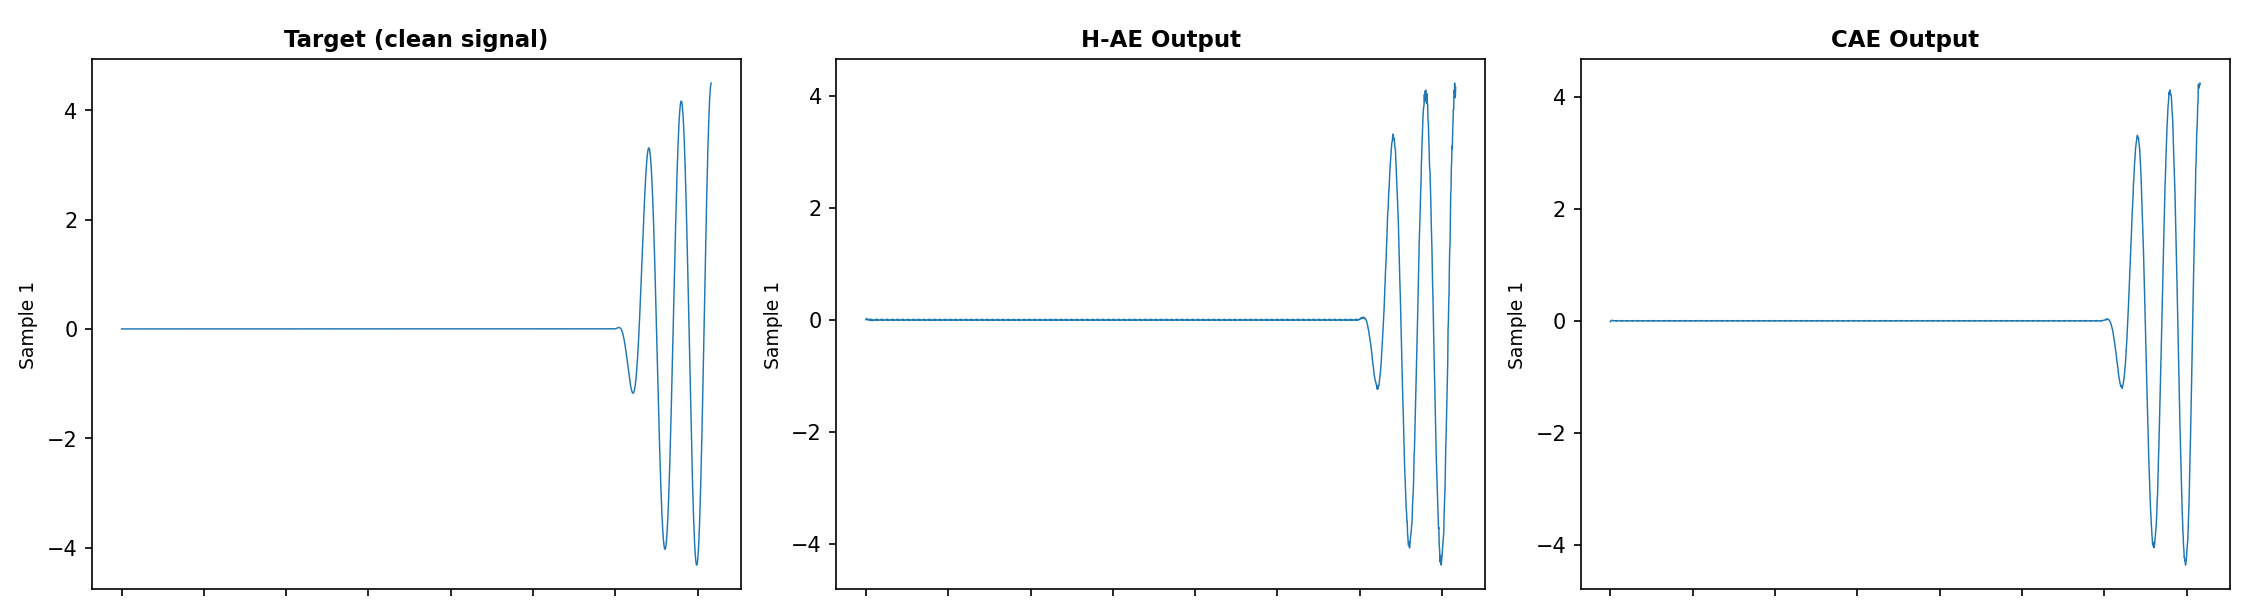
\includegraphics[width=\linewidth]{figures/reconstruction-final.png}
    \caption{Reconstruction of an out-of-sample heavy BBH waveform. Both the CAE and HAE learned the waveform behaviour and their discrepancies are not visually perceptible.}
    \label{fig:reconstruction}
\end{figure}

Both models also clearly capture the inspiral chirp visually and differences in approximation are not visually perceptible. Both of these results were expected, as learning the clean signal is a relatively easy task. Interestingly, the HAE improves on the CAE by \~27\% percent in the test MSE. However, in the training data the CAE has a five-fold lower MSE. This result serves as a partial confirmation to the originally framed hypothesis. The CAE achieves lower training loss because it is optimized to reconstruct the objective, while the HAE must satisfy both loss terms. However, when tested on out-of-sample heavy BBH waveforms it hasn't seen before, it performs worse than the HAE. This indicates that the physics prior restricts the encoder to a constrained family of representations that, although harder to fit, transfer better to out-of-sample events with the same physics.

\subsection{Effect of $\lambda_{phys}$}
Three HAE models were trained with $\lambda \in \{0.01, 0.1, 1\}$. Results for each are for the best hyper parameters for the particular $\lambda$. The CAE is a $\lambda = 0$ baseline, also evaluated at the best respective hyper parameters. Results are in Table~\ref{tab:lambda_sweep}.

\begin{table}[H]
    \centering
    \small
    \caption{Effect of the physics-loss weight $\lambda_{\text{phys}}$ on reconstruction fidelity, waveform overlap, and latent compactness. All metrics computed on test data.}
    \label{tab:lambda_sweep}
    \begin{tabular}{lccc}
        \toprule
        Model & Test MSE  & Overlap  & PC1 ratio \\
        \midrule
        CAE (baseline)               & $2.98 \times 10^{-4}$ & $0.99986$            & $0.672$ \\
        \midrule
        H-AE  $\lambda{=}0.01$       & $1.19 \times 10^{-3}$ & $0.99946$            & $0.582$ \\
        H-AE  $\mathbf{\lambda{=}0.1}$        & $\mathbf{2.17 \times 10^{-4}}$ & $\mathbf{0.99990}$ & $\mathbf{0.697}$ \\
        H-AE  $\lambda{=}1.0$        & $1.16 \times 10^{-3}$ & $0.99948$            & $0.564$ \\
        \bottomrule
    \end{tabular}
\end{table}

All three metrics assessed are not monotonic. For $\lambda=0.01$ the HAE is effectively a CAE and, results wise, is indistinguishable, from a poorly trained CAE. The test MSE, waveform overlap, and PC1 are all worse than the baseline.
For $\lambda=0.1$ the HAE dominates the CAE in every metric. For $\lambda = 1$, it collapse back roughly to $\lambda=0.01$ performance. This is interesting because a generic regularizer degrades monotonically with performance --- $\lambda$ does not.
Instead, the relative weight of Hamiltonian loss exhibits a peak optimum, indicating that this is not simply adding noise to the loss landscape. At too low $\lambda$, the encoder ignores the constraint. At too high of a $\lambda$, the physics term is prioritized over reconstruction, at which \textit{some} scalar is trivially conserved at the cost of representation. The existence of an interior optimum supports the hypothesis: a Hamiltonian structure can be learned in the latent space of a BBH inspiral autoencoder.

\subsection{Latent Space Representation}

The comparisons use the validation-optimal HAE ($\lambda_{phys} = 0.1$) against the CAE baseline (refer to Effect of $\lambda_{phys}$).

PCA (principal component analysis) is a linear dimensionality reduction technique that finds in the data along which variance is largest and re-expresses data in terms of those directions. For each test sample, the latent trajectory is treated as $T_{latent} \times channels$ matrix, and the PCA is run along the time dimension. The higher the PC1 ratio, the lower the degrees of freedom of movement of the system.
The CAE produced a PC1 ratio of 0.672, the HAE --- a ratio of 0.697 (a \~3.7\% improvement). Under the Hamiltonian constraint, a slightly larger fraction of the latent trajectory's variance is concentrated onto the leading direction. This is the behaviour we are expecting if the constraint shaped the latent space toward a 1D-phase-like manifold.
While the change is minor, it is significant because: (i) the CAE is already a strong baseline because the input itself is one-dimensional and quasi-periodic, and (ii) HAE achieves compression \textbf{and} reduces reconstruction error, indicating that this is not a fidelity versus interpretability gain.

\begin{figure}[h]
    \centering
    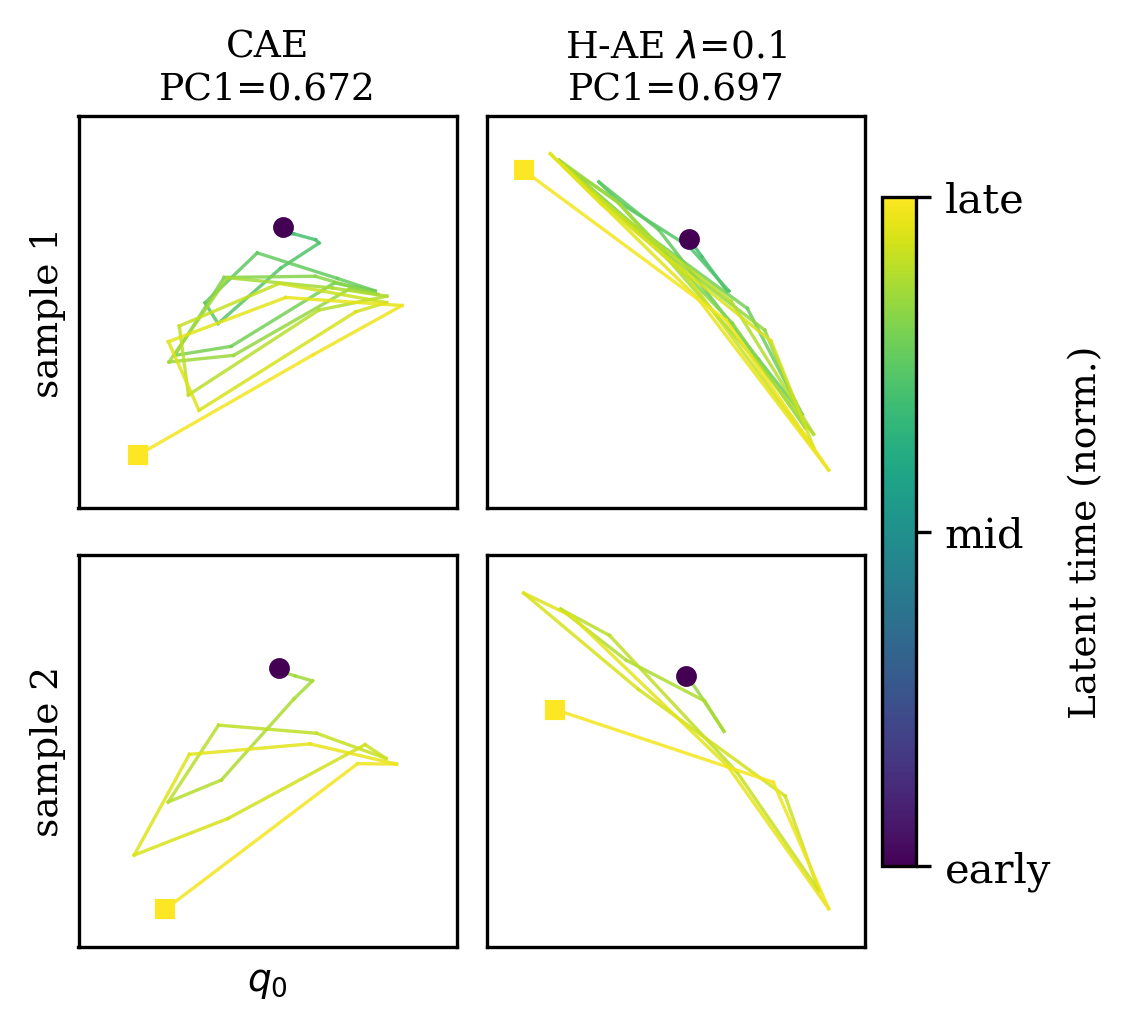
\includegraphics[width=\linewidth]{figures/phase_space_cae_vs_hae.png}
    \caption{The representation of 2 out-of-sample gravitational waves in the latent space for the CAE and H-AE ($\lambda_{phys}=0.1$) for position $q_0$ against $p_0$ for the first canonical pair (out of the two).}
    \label{fig:phase_space}
\end{figure}
Visually, too, the phase-space graphs confirm expectations (refer to Fig.~\ref{fig:phase_space}). The CAE trajectories are diffuse and have a less evident coherent structure. The HAE trajectories are smoother with a coherent structure that is much easier to identify.

This is a particularly interesting result as the variance-of-H formulation is a weaker one than the one employed in Hamiltonian Neural Networks by Greydanus et al \cite{Greydanus2019}.
Together with the $\lambda_{phys}$ sweep, the latent-space analysis supports the thesis that a physics-informed autoencoder trained on BBH gravitational waves is able to find a more compact latent space representation while providing more accurate and transferable results.

% ===========================================================================

% ===========================================================================
\section{Conclusion}
The purpose of this project was to determine whether BBH gravitational waves can be meaningfully represented in a latent space with a physics-informed Hamiltonian loss function and whether this representation improves generalization to out-of-sample waveforms. I determined that the HAE (at $\lambda=0.1$) generalizes better than an identical CAE with a \~27\% lower MSE reconstruction loss. Additionally, the physics prior ($\lambda$) was validated as performance optimum was found in-between extremes, confirming that the Hamiltonian loss acts as a true constraint and not a regularizer. Moreover, the physics constrained increased PC1 compared to the CAE, successfully demonstrating more compact shaping of the latent space. Lastly, the novel use of a variance-of-H loss formulation successfully enforced energy conservation without the need for second-order backpropagation.

% ===========================================================================
\bibliographystyle{IEEEtran}
\bibliography{bib}

\end{document}
